\section{Evaluation}
\label{sec:evaluation}

\begin{table}[t]
  \centering
  \caption{\textbf{Text language model evaluation}. Performance on standard benchmarks for evaluating large language models, including closed book question answering, reasoning and multiple choice QA exams. We report in bold the best performing model trained on less than 2.5T tokens.
  \label{tab:llm_eval}}
  \footnotesize
  \begin{tabular}{lcccccccccc}
    \toprule
    & ARCe & ARCc & OBQA &  HS  &  WG  & PIQA & SIQA & TQA  &  NQ  & MMLU \\
    \midrule
    \helium & \textbf{79.6}  & \textbf{55.9}  & 53.6 & 76.3 & \textbf{70.0} & 79.4 & \textbf{51.0} & \textbf{59.9/72.6} & 23.3 & \textbf{54.3} \\
    \midrule
    MPT     & 70.5  & 46.5  & 51.4 & \textbf{77.6} & 69.9 & \textbf{80.6} & 48.5  & -/61.2 & 20.8 & 30.8 \\
    Falcon  & 73.7  & 47.5  & 53.0 & 76.3 & 68.9 & 80.3 & 47.2 & -/64.6 & 21.0 & 28.0 \\
    Llama 2  & 75.2  & 45.9  & \textbf{58.6} & 77.2 & 69.2 & 78.8 & 48.3 & -/72.1 & \textbf{25.7} & 45.3 \\
    OLMo    & 67.2  & 42.5  & 50.0 & 75.5 & 69.8 & 77.5 & -  & -/- & -  & 52.0 \\
    \midrule
    Mistral & 80.5  & 54.9  & 52.2 & 81.0 & 74.2 & 82.2 & 47.0$^*$ & 62.5/- & 23.2 & 62.5 \\
    Gemma 1  & 81.5  & 53.2  & 52.8 & 81.2 & 72.3 & 81.2 & 51.8 & 63.4/- & 23.0 & 64.3 \\
    \bottomrule
  \end{tabular}%
\end{table}

\subsection{Text Language Modeling}
\label{sec:helium_eval}
\paragraph{Metrics.}
We evaluate \helium (trained only on text data) on the following standard benchmarks: AI2 Reasoning Challenge~\citep[ARC]{clark2018think}, Open-Book QA~\citep[OBQA]{mihaylov2018can}, HellaSwag~\citep[HS]{zellers2019hellaswag}, WinoGrande~\citep[WG]{sakaguchi2021winogrande}, Physical Interaction QA~\citep[PIQA]{bisk2020piqa}, Social Interaction QA~\citep{sap2019socialiqa}, TriviaQA~\citep[TQA]{joshi2017triviaqa}, Natural Questions~\citep[NQ]{kwiatkowski2019natural} and Massive Multitask Language Understanding benchmark~\citep[MMLU]{hendrycks2020measuring}.
These benchmarks cover a wide variety of tasks, including common sense reasoning, closed-book question answering or multiple choice question answering from high school and college subjects.
We follow the evaluation protocol from previous work such as GPT-3 or Llama: we perform 5-shot evaluation on TriviaQA, NQ and MMLU, and 0-shot evaluation on the other datasets.
On TriviaQA, we report performance on the Unfiltered and Wikipedia splits.

\paragraph{Baselines.}
As baselines, we consider existing large language models with a size around 7B parameters, and which are trained using roughly the same amount of compute as Helium.
More specifically, we include models that are trained on fewer than 2.5T tokens (compared to the 2.1T tokens that are used to train Helium), namely MPT~\citep{MosaicML2023Introducing}, Falcon~\citep{almazrouei2023falcon}, Llama 2~\citep{touvron2023llama} and OLMo~\citep{Groeneveld2023OLMo}.
We also include Mistral and Gemma, two popular open weights models that are trained using significantly more compute than \helium.

\paragraph{Results.}
We report results in \hyperref[tab:llm_eval]{Table~\ref{tab:llm_eval}}, and we observe that on most benchmarks, Helium is on-par or outperforming models using similar amount of training compute.
Even compared to Mistral and Gemma, which use up to 3x more compute for training, Helium obtains competitive results on some benchmarks such as ARC, Open-Book QA or Natural Questions.
This validates the quality of our pre-training text data.






\subsection{Audio Tokenization}
\label{sec:mimi_eval}

\looseness=-1
\paragraph{Metrics.}
We then evaluate the semantic and acoustic performance of our neural codec, \mimi. First, we evaluate whether the semantic tokens it produces provide targets that are amenable to language modeling. To do so, we compute a triphone-based ABX~\citep{abx} error rate that characterizes the phonetic discriminability of a representation space by comparing distances between two embeddings of different instances of a same triphone (e.g.``beg'') and a negative triphone that differs minimally (e.g.``bag''). More precisely, we compute a ``within speaker" ABX where the three instances are pronounced by the same speaker, and report error rates on Librispeech~\citep{librispeech} dev-clean with the default parameters of the Librilight \citep{librilight} repository\footnote{\url{https://github.com/facebookresearch/libri-light/blob/main/eval/README.md}}. The resulting score has been shown to be a strong predictor of the ability of a downstream audio language model to produce coherent speech~\citep{gslm}. Since we are interested in characterizing only the semantic token, we compute distances in the latent space produced after quantization with the semantic VQ only (i.e. before summing with acoustic tokens). 
\looseness=-1
Second, we evaluate the acoustic quality of reconstructed audio. As objective, automatic metrics we rely on VisQOL~\citep{hines2015visqol}--- a full-reference model of acoustic similarity--- and MOSNet~\citep{mosnet}--- a reference-free model of audio quality. Given the limitations of automatic evaluation of audio quality, we also perform human evaluations with a MUSHRA protocol. We rely on judgments of 20 listeners, each one rating 30 samples of 10s each. \hyperref[tab:mimi_ablations]{Table~\ref{tab:mimi_ablations}} reports ablations studies using objective metrics, while \hyperref[tab:mimi_baselines]{Table~\ref{tab:mimi_baselines}} provides a comparison with previous work both in terms of objective and subjective evaluation.

\paragraph{Baselines.}
We compare against RVQGAN~\citep{kumar2024high}, SemantiCodec~\citep{liu2024semanticodec}, and SpeechTokenizer ~\citep{zhang2024speechtokenizer}. RVQGAN is a pure acoustic tokenizer, in the sense that it does not encode semantic information. Thus, we only evaluate it in terms of audio quality. RVQGAN produces tokens at 75Hz, so we only keep the first two levels of RVQ to obtain a bitrate of 1.5kbps, closer to that of \mimi{}. On the other hand, SpeechTokenizer relies on distillation to encode semantic information into its first token such that we can evaluate both its semantic and acoustic properties. We keep its first 3 RVQ levels to obtain a 1.5kbps bitrate. Similarly, SemantiCodec also encodes semantic and acoustic information such that it can be evaluated along both axes.



\begin{table}[t]
  \centering
  \caption{\textbf{Ablation study on hyper-parameters of the \mimi codec}. We evaluate semantic modeling by reporting the error rate on a phonetic ABX discriminability task. To evaluate the reconstruction quality, we compute VisQOL and MOSNet and collect human judgments with a MUSHRA protocol. ``Quantization rate'' refers to applying quantization to the latent space only $50\%$ of the time during training (independently from quantizer dropout), as described in \hyperref[sec:mimi]{Section ~\ref{sec:mimi}}.}
  \label{tab:mimi_ablations}
  \resizebox{\textwidth}{!}{
  \begin{tabular}{ccccc|cccc}
    \toprule
    Quantization & Transformer & Transformer & WavLM & Split & \multirow{2}{*}{ABX ($\downarrow$)} & \multirow{2}{*}{VisQOL ($\uparrow$)} & \multirow{2}{*}{MOSNet ($\uparrow$)} & \multirow{2}{*}{MUSHRA ($\uparrow$)} \\
    Rate & in encoder & in decoder & distillation & quantizer &  &  &  \\
    \midrule
     \checkmark & \checkmark & \checkmark & \xmark & \xmark & 23.3\% & 2.91 & 2.89 & 65.9\pmr{1.7}\\ %
     \checkmark & \checkmark & \checkmark & \checkmark & \xmark & 6.5\% & 2.22 & 2.87 & 57.8\pmr{1.8} \\ %
     \checkmark & \xmark & \checkmark & \checkmark & \checkmark & 10.8\% & 2.79 & 2.85 & 59.7\pmr{1.7} \\ %
     \checkmark & \checkmark & \xmark & \checkmark & \checkmark & 8.1\% & 2.59 & 2.72 & 48.4\pmr{1.7} \\ %
     \xmark & \checkmark & \checkmark & \checkmark & \checkmark & 8.0\% & 2.45 & 2.88 & 68.3\pmr{1.7} \\ %
     \checkmark & \checkmark & \checkmark & \checkmark & \checkmark & 8.1\% & 2.82 & 2.89 & 64.0\pmr{1.7} \\ %
    \bottomrule
  \end{tabular}
  }
\end{table}

\begin{table}[t]
  \centering
  \caption{\textbf{Audio quality evaluation}. Objective and subjective (MUSHRA) evaluation of audio quality for baseline neural audio codecs---RVQGAN~\citep{kumar2024high}, SemantiCodec~\citep{liu2024semanticodec}, and SpeechTokenizer ~\citep{zhang2024speechtokenizer}--- and the most important variants of \mimi. For a fair comparison with SemantiCodec and SpeechTokenizer, we also include a downsampled version of our codec in the MUSHRA study. $f_s$ is the audio sample rate and $f_r$ the codec frame rate. Both \mimi codecs are trained with distillation, and either with the same combination of reconstruction and adversarial losses as Encodec (see \hyperref[sec:mimi]{Section~\ref{sec:mimi}}) or adversarial losses only.}
  \label{tab:mimi_baselines}
  \resizebox{\textwidth}{!}{
  \begin{tabular}{lcccc|ccc|c}
    \toprule
    Model & $f_s$ & $f_r$ & bitrate & causal & ABX ($\downarrow$) & VisQOL ($\uparrow$) & MOSNet ($\uparrow$) & \textsc{MUSHRA} ($\uparrow$) \\
    \midrule
    Ground Truth & 24kHz & - & - & - & - & - & 3.08 & 90.6\pmr{1.0}\\
    \midrule
    RVQGAN & 24kHz & 75Hz & 1.5kbps & \xmark & - & 1.74& 2.74 & 31.3\pmr{1.3}\\
    SemantiCodec & 16kHz & 50Hz & 1.3kbps & \xmark & 42.2\% & 2.43 & 3.12 & 64.8\pmr{1.5} \\
    SpeechTokenizer & 16kHz & 50Hz & 1.5kbps & \xmark & \textbf{3.3\%} & 1.53 & 2.67 & 45.1\pmr{1.5} \\
    SpeechTokenizer & 16kHz & 50Hz & 4.0kbps & \xmark & \textbf{3.3\%} & 3.07 & 3.10 & 74.3\pmr{1.5} \\
    \midrule
     Mimi, adv. loss only & 24kHz & 12.5Hz & 1.1kbps & \checkmark & 8.7\% & 1.84 & 3.10 & \textbf{81.0}\pmr{1.3} \\
     Same, downsampled at 16kHz & 16kHz & 12.5Hz & 1.1kbps & \checkmark & - & - & - & 77.7\pmr{1.4}\\
     Mimi, non adv. only& 24kHz & 12.5Hz & 1.1kbps & \checkmark & 8.1\% & 2.82 & 2.89 & 58.8\pmr{1.8}\\
    \bottomrule
  \end{tabular}}
\end{table}



\looseness=-1
\paragraph{Results - Semantic tokens.} \hyperref[tab:mimi_ablations]{Table~\ref{tab:mimi_ablations}} shows that \mimi's phonetic discriminability of semantic tokens, as measured by ABX, is poor in the absence of distillation and comparable to acoustic tokens of previous work~\citep{audiolm}: This means these semantic tokens are not amenable to capturing linguistic content from speech. In contrast, distilling WavLM into the semantic tokens significantly improves their phonetic discriminability, in particular when using a Transformer in \mimi's encoder. This can be explained by the fact that distilling a large Transformer based encoder into a purely convolutional one is challenging, while increasing the capacity and receptive field of the encoder helps. Yet,  we observe a conflict between acoustic losses and semantic distillation, as improving ABX implies reducing reconstruction quality (as measured by MUSHRA). Using a split RVQ as described in \hyperref[sec:splitrvq]{Section~\ref{sec:splitrvq}} improves the trade-off between semantic properties and audio quality, improving MUSHRA from 57.8 to 64.0 while moderately degrading ABX from 6.5\% to 8.1\%.


\looseness=-1
\paragraph{Results - Acoustic tokens.} \hyperref[tab:mimi_ablations]{Table~\ref{tab:mimi_ablations}} also shows a significant improvement in MUSHRA when adding a Transformer in the decoder. Similarly, using a quantization rate of $50\%$ significantly improves VisQOL.  Quantization rate however does not improve perceived quality. More generally, we observe a poor correlation between VisQOL and MOSNet. In particular, \hyperref[tab:mimi_baselines]{Table~\ref{tab:mimi_baselines}} shows that training \mimi with adversarial losses only leads to a very low VisQOL of 1.84 which does not account for the high perceived audio quality. We thus rely on MUSHRA where raters are asked to judge the similarity of a reconstructed audio to its ground-truth anchor, with a score between 0 and 100. This human evaluation shows a significant improvement from using adversarial losses only, with a MUSHRA score of 81.0 against 58.8 when using the mix of loss functions used in Encodec. \mimi moreover significantly outperforms RVQGAN~\citep{dac} despite operating at a lower bitrate and modeling semantic information. \mimi also provides higher reconstruction quality than SemantiCodec~\citep{liu2024semanticodec} while operating at a 4$\times$ lower framerate. This property is crucial to achieve the low latency of \ours{}, since generating one temporal frame of audio tokens with \ours{} requires a full forward pass through the Temporal Transformer. Finally, both RVQGAN and SemantiCodec are non-causal, while \mimi is fully causal and thus compatible with streaming inference and modeling of real-time conversations.

\looseness=-1
\paragraph{Discussion.}
\mimi overall provides high reconstruction quality while encoding semantic information, being fully causal, and operating at low framerate and bitrate. In consequence, \mimi proves to be a well-fitted audio tokenizer to train real-time audio language models. A collateral finding of our study is a concerning lack of correlation between objective and subjective audio quality metrics. In particular, while we find VisQOL to provide a reliable proxy for perceived quality when modifying the generator architecture, changing the training objective (e.g. removing reconstruction losses) moves the score in directions that are completely decorrelated from human perception. This observation underscores the open challenge of designing reliable objective proxies for perceived quality.

\begin{table}[t]
    \small	
    \centering
    \caption{
    \textbf{Ablation study on the use of the RQ-Transformer}. All models are initialized with Helium and pretrained on audio. When not using RQ-Transformer, we predict the 8 levels of tokens with independent classification heads, following~\citet{musicgen}. Note that perplexities are only comparable between models with a given delay, as the classification task is easier with more delay for higher tokens.}
    \footnotesize
    \begin{tabular}{ccc}
    \toprule
     Acoustic Delay & RQ-Transformer & Perplexity \\
     \midrule
    $[0, 1, 2, 3, 4, 5, 6, 7]$ & \xmark &  $\phantom{1}42.2$ \\
    $[0, 1, 2, 3, 4, 5, 6, 7]$ & \checkmark &  $\phantom{1}40.3$ \\
    $[0, 2, 2, 2, 2, 2, 2, 2]$ & \xmark &  $135.4$\\
    $[0, 2, 2, 2, 2, 2, 2, 2]$ & \checkmark & $\phantom{1}36.8$ \\
    \bottomrule
    \end{tabular}
    \label{tab:ablation-rq}
\end{table}

\begin{table}[t]
    \small
    \centering
    \caption{
      \textbf{Ablation study on delay patterns, weight of the semantic token and \interleaving{}}. All models are initialized with Helium, pretrained on audio and use the RQ-Transformer. We vary the weight of the semantic token while keeping the weight of other tokens (including the text token when using \interleaving{}) to 1. As different delay patterns cannot be compared in terms of perplexity, we generate continuations from 3s prompts on the valid set, convert them into transcripts with Whisper~\citep{whisper} and report their negative log-likelihood with LiteLlama-460M-1T\protect\footnote{\url{https://huggingface.co/ahxt/LiteLlama-460M-1T}} along with their length (in characters) as proxies for linguistic quality.}
      \footnotesize
    \begin{tabular}{cccccrr}
    \toprule
     Acoustic & Semantic Token & Depthwise & Inner & Transcript  & Transcript \\
      Delay & Weight & Parametrization & Monologue & NLL ($\downarrow$) & Length ($\uparrow$)  \\
     \midrule
    $[0, 0, 0, 0, 0, 0, 0, 0]$ & \phantom{00}1.0 & \cmark & \xmark & $4.36$ & $486$ \\
    $[0, 1, 1, 1, 1, 1, 1, 1]$ & \phantom{00}1.0 & \cmark & & $4.12$ & $529$ \\
    $[0, 2, 2, 2, 2, 2, 2, 2]$ & \phantom{00}1.0 & \cmark & & $4.09$ & $519$ \\
    $[0, 2, 2, 2, 2, 2, 2, 2]$ & 100.0 & & & $3.75$ & $538$ \\
    $[0, 2, 2, 2, 2, 2, 2, 2]$ & 100.0 & \cmark & & $3.65$ & $602$ \\
    $[0, 2, 2, 2, 2, 2, 2, 2]$ & 100.0 & \cmark & \cmark & \textbf{2.77} & \textbf{1920} \\
    \bottomrule
    \end{tabular}
    \label{tab:ablation-delays}
\end{table}

\subsection{Ablations on Generative Modeling}
\label{sec:moshi_ablations}
\paragraph{Metrics.} We perform ablation studies to evaluate the impact of using an RQ-Transformer, as well as comparing delay patterns and weighting of various token levels. All models are initialized with \helium{} for the Temporal Transformer and pretrained on audio data. When comparing models with a same delay pattern and without \interleaving{}, we rely on perplexity, averaged over semantic and acoustic tokens. However, perplexities are not comparable between models with various delays, as they do not model the same conditional distributions. To compare various delay patterns, we measure the ability of \ours{} to generate intelligible, consistent speech by transcribing generations (conditioned on a 3s prompt) with Whisper~\citep{whisper} and scoring the resulting transcripts with an external text language model. We rely on a lightweight text model---LiteLlama-460M-1T\footnote{\url{https://huggingface.co/ahxt/LiteLlama-460M-1T}}--- as it is more practical for continuous evaluation along training. We also report the length of the transcripts (in characters), as we find it to a be a strong predictor of model quality (weak models typically collapse to silence).

\paragraph{Results - RQ-Transformer.} \hyperref[tab:ablation-rq]{Table~\ref{tab:ablation-rq}} reports results for ablations on the use of an RQ-Transformer. We first replicate the setting of \citet{musicgen} with the delay pattern of $[0, 1, 2, 3, 4, 5, 6, 7]$, which means that each level of RVQ token is generated one timestep after the preceding level. In this context, we see that using an RQ-Transformer is not necessary, as it only provides a marginal improvement in perplexity. However, this delay pattern induces a theoretical latency of 8 timesteps, which amounts to 640ms, a latency that is incompatible with the requirements of a real-time dialogue model. We thus switch to a reduced latency of 240ms with the pattern $[0, 2, 2, 2, 2, 2, 2, 2]$. In that context, modeling RVQ tokens with an RQ-Transformer significantly improves perplexity over using separate classification heads. Thus, the RQ-Transformer becomes a critical component of generative models of RVQ tokens under strict latency constraints.

\paragraph{Results - Additional ablations.} \hyperref[tab:ablation-delays]{Table~\ref{tab:ablation-delays}} reports additional ablations on additional delay patterns, the weight of the semantic token loss and our proposed Inner Monologue procedure, all using the RQ-Transformer. 
First, we compare three configurations of delays that are compatible with real-time dialogue. The $[0, 0, 0, 0, 0, 0, 0, 0]$ pattern represents the minimal latency of 80ms that can be obtained with \mimi{} tokens at 12.5Hz. Allowing an additional 80ms of latency with one step of delay significantly improves the quality of generated speech, while 240ms of latency brings further moderate improvement. 
In early experiments, we also observed that the individual losses per RVQ level were conflicting with one another, despite each level being more important in the final intelligibility and audio quality than the next one. We thus bring two changes to the architecture and training process. We first increase the weight of the loss on predicting the semantic tokens to 100, while keeping it at 1 for all other levels of the audio tokens. 
This gives another boost to speech intelligibility. We furthermore reduce competition between RVQ levels by using a depthwise parametrization, as described in \hyperref[sec:joint_ar]{Section~\ref{sec:joint_ar}}, such that each RVQ level is predicted by its own set of weights in the Depth Transformer, rather than having shared weights across levels.
Finally, the most drastic improvement to the quality and length of generated speech comes from enabling \interleaving{}.

\looseness=-1
\paragraph{Discussion.} Beyond the choice of architecture and delay patterns, these ablations show how helpful modeling text tokens along the audio tokens with \interleaving{} is, even in an audio-to-audio setting. Given the positive impact of depthwise parametrization and a weight of 100 for the semantic token, both are used in the subsequent experiments and our final training procedure. As described in \hyperref[tab:hparams]{Table~\ref{tab:hparams}}, we pretrain \ours{} with an acoustic delay of 2 and finetune it with an acoustic delay of 1, for a theoretical latency of 160ms.

\begin{table}[t]
    \centering
    \caption{\textbf{Performance of audio and text language modeling}. We report accuracies based on scoring with negative log-likelihood, normalized by sequence length. MMLU is evaluated in a 5-shot setting. Reusing the terminology of \cite{spiritlm}, $\varnothing$ represents unsupported modalities while - represents unreported numbers.}
    \resizebox{\textwidth}{!}{  
    \begin{tabular}{lccccc}
    \toprule
    &
    \multicolumn{4}{c}{Audio metrics} &
    \multicolumn{1}{c}{Text metrics} \\
    \cmidrule{2-5}
    \cmidrule(l){6-6}
     Model & sWUGGY & sBLIMP & sTopic-StoryCloze & sStoryCloze & MMLU \\
    \midrule
    \multicolumn{6}{c}{\textit{Audio only - Cold Start}} \\
    \midrule[0.3pt]
    GSLM \citep{gslm} &  64.8 &   54.2 &  66.6 &  53.3 & $\varnothing$ \\
    AudioLM \citep{audiolm} &  71.5 &   \textbf{64.7} &   - &   - & $\varnothing$ \\
    TWIST \citep{twist} & 72.2 & 56.5 &  - & - & $\varnothing$ \\
    \midrule[0.01pt]
    \ours{} %
    & \textbf{74.8} & 59.9 & 80.9 & 56.9 & $\varnothing$ \\
    \midrule
    \multicolumn{6}{c}{\textit{Audio only - Warm Start}} \\
    \midrule[0.3pt]
    TWIST \citep{twist} & 74.5 & 59.2 & 76.4 & 55.4 & $\varnothing$ \\
    VoxtLM \citep{voxtlm} &  62.9 &   53.9 &   - &   - & $\varnothing$  \\
    Spirit-LM \citep{spiritlm} &  69.5 &   58.0 &   72.9 &   54.8 & $\varnothing$  \\
    \midrule[0.01pt]
    \ours{} %
    & 74.3 & 58.9 & 81.8 & 58.7 & $\varnothing$  \\
    \midrule
    \multicolumn{6}{c}{\textit{Text and audio - Warm Start}} \\
    \midrule[0.3pt]
    VoxtLM \citep{voxtlm} & 66.1 &  57.1 & - & - &  $\varnothing$ \\
    Spirit-LM \citep{spiritlm} & 69.0 & 58.3 & 82.9 & 61.0 & 36.9  \\
    \midrule[0.01pt]
    \ours{} after single-stream pretraining %
    & 72.6 &58.8 & 83.0 & 60.8 & \textbf{49.8} \\
    \ours{} after multi-stream instruct %
    & 63.0 & 55.2 & \textbf{83.6} & \textbf{62.7} & 49.7 \\
    \ours{} after multi-stream instruct, synthetic voice %
    & 60.9 & 54.6 & 82.5 & 60.9 & 48.7 \\
    \bottomrule
    \end{tabular}}
    \label{tab:textless}
\end{table}

\subsection{Audio Language Modeling}
\label{sec:eval_audiolm}
\looseness=-1
\paragraph{Metrics.} We first measure the ability of \ours{} to model speech sequences when being trained for next token prediction on large scale audio data. To do so, we rely on ``textless NLP''~\citep{gslm} metrics that evaluate an audio language model's linguistic knowledge by comparing likelihoods of positive and negative speech examples represented as audio tokens. sWUGGY evaluates a model's ability to learn a lexicon from speech by comparing the likelihood of an existing word and an invalid variant (e.g. ``oxidation'' and ``accidation''), while sBLIMP evaluates syntactic contrasts. Spoken StoryCloze metrics introduced by~\citet{twist} evaluate semantic contrasts by comparing commonsense five-sentence stories, with the last one being either coherent with the context or incoherent. Given the difficulty of this task in the audio domain, \citet{twist} also propose  Spoken Topic-StoryCloze, a variant  where the negative continuation is randomly sampled among unrelated sentences (rather than being subtly incoherent), resulting in higher scores. We score sequences with a negative-log likelihood normalized by the sequence length. Since our model produces several tokens per timestep, we sum all tokens of a timestep with the weights used during training, i.e. 100 for the semantic tokens and 1 for the acoustic ones. We do not include text tokens from the \interleaving{}, as these metrics are designed to compare untranscribed audio sequences. Similarly, when evaluating a multi-stream model after instruction tuning, we only score the tokens from the user stream as it does not include text tokens. Finally, we also report text understanding  evaluation (without audio tokens) on MMLU~\citep{hendrycks2020measuring} for Spirit-LM and \ours{}, as a way to measure how much the audio training affects the textual knowledge of the original checkpoint.
\looseness=-1
\paragraph{Baselines.} We compare against baselines from the audio language modeling literature, in three settings. The first category encompasses audio-only models starting from a random initialization, including GSLM~\citep{gslm}, AudioLM~\citep{audiolm} and TWIST-1.3B~\citep{twist}. In this case, we report metrics for a single-stream \ours{} initialized randomly and pretrained only on audio data and without \interleaving{}. The second category includes models that start from a pretrained text LM and are then only trained on audio. This includes TWIST-13B as well as the audio-only version of VoxtLM (first row of \citep[Table 3]{voxtlm}) and that of Spirit-LM (reported as ``Speech Only'' in \citep[Table 5]{spiritlm}). The corresponding \ours{} model is similar to the one mentioned above (audio-only data, no \interleaving{}) but starts from the pretrained \helium{} checkpoint. The last category is composed of actual multimodal models that are trained jointly on speech and text data. In this context we report results for three configurations of \ours{}. First, we report results for \ours{} pretrained on single-stream data. Then, we report results for the final model after multi-stream post-training and finetuning using real recordings from a voice actor to condition the creating of synthetic data in Moshi's voice. The last model is identical to the previous one except for the fact that it uses a synthetic voice for \ours{}. We remind the reader that even if these models are trained with \interleaving{}, they are evaluated without, to provide a fair comparison with baselines.
\looseness=-1
\paragraph{Results.} \hyperref[tab:textless]{Table~\ref{tab:textless}} reports results on audio language modeling. In the ``Audio only - Cold Start'' setting, \ours{} already provides a strong baseline, in particular considerably improving over previous work in sTopic-StoryCloze.  When initialized with an \helium{} checkpoint and trained on audio-only data, \ours{} outperforms previous work in this category on most metrics. Finally, while multimodal training improves common sense reasoning from speech (as shown by sStoryCloze performance), we observe mixed effects on lexical and syntactic judgments (sWUGGY and sBLIMP) compared to models trained only on audio data. While single-stream pretraining moderately degrades sWUGGY and sBLIMP, instruction finetuning severely affects sWUGGY, which means that instructed models have a harder time solving lexical judgments. 
We hypothesize that this is due to finetuning \ours{} on data of varying quality and simulating noisy and reverberated conditions for the user stream (used to score spoken pairs for all metrics in \hyperref[tab:textless]{Table~\ref{tab:textless}}) which makes fine lexical judgments harder to solve. Finally, Moshi scores 12 points higher on MMLU than Spirit-LM, thus demonstrating higher general knowledge and text understanding. We moreover emphasize that \ours{} is the only model in \hyperref[tab:textless]{Table~\ref{tab:textless}} that integrates both semantic and acoustic tokens into a single generative model, unlike AudioLM which uses three separate stages, and VoxTLM, TWIST and Spirit-LM that only model semantic tokens and rely on an external vocoder. Thus, \ours{} is the only model in this comparison that demonstrates strong linguistic modeling in both speech and text, while being able to model speech in any arbitrary voice and condition.

\paragraph{Discussion.}
\looseness=-1
While ``textless NLP'' benchmarks have helped developing the first audio language models, we observe that they do not consistently provide good guidance in developing a dialogue model like \ours{}. In particular, we find the lack of correlation between common sense metrics and lexical/syntactic judgments to be frequent and easily explainable by the diversity of acoustic conditions we use in training. Moreover, we do not observe a degradation in the model's lexical variety or intelligibility when finetuning the model, which contradicts the reduction in sWUGGY. This is why we also evaluate spoken question answering in the next section as a way to probe the model's common sense, knowledge and lexical abilities.

\begin{table}
    \footnotesize	
    \centering
    \caption{\textbf{Evaluation of spoken question answering}.
    Spoken question answering (0-shot) on the Web Questions~\citep{web_questions}, LlaMA-Questions~\citep{spectron}, and Trivia QA~\citep{joshi2017triviaqa} benchmarks, synthesized using a TTS engine.
    For the first two, we use the number reported by~\citep{spectron}.
    For LlaMA-Questions, we use the audio provided by~\citep{spectron}.
    For Web Questions and Trivia QA, we synthesize our own, keeping all of the questions. For \ours{}, we only prepend one of the random incipits used during instruct fine tuning. We further provide the performance
    of our \helium text-only model as a top line.}
    \begin{tabular}{lccc}
    \toprule
     Model & Web Q. & LlaMA Q. & Audio Trivia QA\\
    \midrule
    \multicolumn{4}{c}{\textit{Audio only}} \\
    \midrule[0.3pt]
    GSLM \citep{gslm} & \hphantom{0}1.5 &  \hphantom{0}4.0 &   - \\
    AudioLM \citep{audiolm} & \hphantom{0}2.3 & \hphantom{0}7.0 &   - \\
    TWIST (7B) \citep{twist} & \hphantom{0}1.1 & \hphantom{0}0.5 &   - \\
    \midrule[0.01pt]
    \ours (w/o \interleaving{}) & \hphantom{0}\textbf{9.2} & \textbf{21.0} & 7.3   \\
    \midrule
    \multicolumn{4}{c}{\textit{Text and audio}} \\
    \midrule[0.3pt]
    SpeechGPT (7B) \citep{zhang2024speechgpt} & \hphantom{0}6.5 & 21.6 &   14.8 \\
    Spectron (1B) \citep{spectron} & \hphantom{0}6.1 & 22.9 &   - \\
    \midrule[0.01pt]
    \ours & \textbf{26.6} & \textbf{62.3} &   \textbf{22.8} \\ %
    \ours (w/o text batches in pre-training) & 23.2 & 61.3 &   18.3 \\ %
    \midrule
    \multicolumn{4}{c}{\textit{Text}} \\
    \midrule[0.3pt]
    Helium (text) & 32.3 & 75.0 & 56.4 \\
    \bottomrule
    \end{tabular}%
    \label{tab:qa}
\end{table}

\subsection{Spoken Question Answering}
\looseness=-1
\paragraph{Metrics.} 
We evaluate the spoken question answering abilities of our multi-stream \ours{} model. We rely on Spoken Web Questions and Llama Questions, both introduced by~\citet{spectron}. We also synthesize an audio version of TriviaQA. When evaluating \ours{}, we insert the audio tokens of the question into the user stream to simulate a user interaction, along with a final \texttt{EPAD} text token to trigger an immediate response from \ours{}. 

\paragraph{Baselines.} 
We compare to Spectron and baselines used by~\citet{spectron}, all having been already introduced in \hyperref[sec:eval_audiolm]{Section~\ref{sec:eval_audiolm}} except for SpeechGPT~\citep{zhang2024speechgpt}. To measure the impact of \interleaving{} on spoken fluency, we compare these baselines with \ours{}  trained with and without \interleaving{}. As GSLM, AudioLM and TWIST are audio only, \ours{} without \interleaving{} provides a fair comparison. On the other hand, Spectron and SpeechGPT rely on Chain-of-Modality---they generate an answer first as text, and then as speech--- so we compare them to Moshi with \interleaving{}. Moreover, to quantify an eventual degradation in knowledge due to training on audio data, we also compare to \helium{} when evaluated on the textual counterpart to each spoken dataset.
\looseness=-1
\paragraph{Results.} \hyperref[tab:qa]{Table~\ref{tab:qa}} reports accuracies on the three benchmarks. While audio-only \ours{} significantly outperforms baselines in its categories, the most striking result is the impact of \interleaving{} on Moshi's performance, almost tripling its accuracy on all benchmarks. This is remarkable as \interleaving{} only marginally increases inference cost (each multi-stream timestep requires generating 17 tokens, instead of 16 without). We emphasize that among all models in this comparison, Moshi not only provides the best spoken question answering performance, but is also the only one to model jointly semantic and acoustic tokens, such that it can handle interactions between arbitrary voices in many conditions. \ours{} significantly outperforms SpeechGPT and Spectron while it is the only model compatible with streaming inference, as Chain-of-Modality requires generating a full answer in text before generating speech, while \interleaving{} generates both in a streaming fashion.
Finally, we note that Moshi with \interleaving{} but without keeping 50\% of text-only batches during pre-training leads to a noticeable drop in acccuracy, showing that a warm start from Helium is not sufficient to retain the knowledge of the original text model throughout the training.
\looseness=-1
\paragraph{Discussion.} Despite the strong performance of \ours{}, we observe a weaker performance than the base\helium{} model, which is consistent with the reduced MMLU of 49.7 reported in \hyperref[tab:textless]{Table~\ref{tab:textless}} from 54.3 with \helium{}. While the moderate differences on Web Questions and Llama Questions can be explained by training on audio data and thus reducing the amount of parameters dedicated to textual knowledge, the very large difference on Trivia QA incites us to inspect more thoroughly patterns of errors. We find that multiple-sentence questions (e.g. ``The Terror of the Monster was an early title for a best-selling novel which inspired one of the highest-grossing movies of the mid-70's. Under what name did it eventually terrify the reading and film going public?'') or ones with specific syntactic structure (e.g. ``On the human body, a keloid is a type of what?'') are challenging for \ours{}, due to it being finetuned on oral-style conversations that do not display such patterns. We hypothesize that covering more syntactic scenarios during finetuning could reduce this gap.

\begin{table}[t]
    \footnotesize	
    \centering
    \caption{\textbf{Linguistic quality and turn-taking statistics of generated dialogues}. As we train our multi-stream model to generate both sides of the conversation, we can generate dialogues without the need to interact with a real user. This allows evaluating how much \ours{} learns natural conversational dynamics.}
    \resizebox{\textwidth}{!}{  
    \begin{tabular}{lccccccc}
    \toprule
    Model& samples&temp&cond. PPL& IPU & Pause & Gap & Overlap \\
    \midrule
    Best non-cascaded \citep{nguyen-etal-2023-generative}
    & 50 & 1.0 & 195.9 & 41.4s & 13.8s & 10.7s & 6.1s \\
    Cascaded \citep{nguyen-etal-2023-generative}
    & 50 & 1.0 & 45.9 & 54.8s & 0.0s & 5.3s & 0.0s \\
    Ground Truth \citep{nguyen-etal-2023-generative}
    & 50 & $\varnothing$ & 65.0 & 53.5s & 5.5s & 4.4s & 3.6s \\
    \midrule
    \ours{} %
    & 1000 & 0.8 & \textbf{41.9} & 35.1s & 13.2s & 12.5s & 1.2s \\
    \ours{} %
    & 1000 & 0.9 & 56.7 & 44.7s & 9.1s & 7.5s & 2.2s \\
    \ours{} %
    & 1000 & 1.0 & 79.3 & 50.8s & 7.0s & 4.5s & 4.1s \\
    Ground Truth 
    & 1000 & $\varnothing$ & 59.6 & 51.1s & 6.4s & 4.2s & 3.3s \\
    \bottomrule
    \end{tabular}
    }
    \label{tab:multistream}
\end{table}

\subsection{Quality and Statistics of Generated Dialogues}
\label{sec:eval_dialogues}
\paragraph{Metrics.}
\looseness=-1
Beyond single-turn question answering, we evaluate the linguistic quality of the generated dialogues by scoring them with an external language model, while also looking at turn-taking metrics. We follow the methodology of ~\citet{nguyen-etal-2023-generative}. The turn-taking metrics are defined as follows: \emph{Inter-Pausal Units} (IPU) are continuous streches of speech that are separated by a silence of at least 0.2s on each side.
\emph{Pauses} are silences between IPUs of the same speakers.
\emph{Gaps} are silences between IPUs of different speakers.
\emph{Overlaps} are times where there are IPUs for both speakers. Following ~\citet{nguyen-etal-2023-generative}, the semantic evaluation uses the open-source DialoGPT model~\cite{dialogpt} and we compute the perplexity of the transcribed dialogue by separating each speaker using the \texttt{<|endoftext|>} token expected by DialoGPT.
We select 1000 random 10 seconds prompts from the Fisher dataset and use \ours{} to generate continuations. For each one, 32 continuations are generated, for
3 different temperatures as it significantly affects the results.

\paragraph{Baselines.} We compare to dGSLM \citep{nguyen-etal-2023-generative}, as it is also a full-duplex generative model, trained on the Fisher dataset. \citet{nguyen-etal-2023-generative} use 50 prompts with 50 continuations for each and report results for their dialogue model as well as a cascaded topline model (ASR + LM + TTS).

\paragraph{Results.} \hyperref[tab:multistream]{Table~\ref{tab:multistream}} shows that \ours{} performs as well as the cascaded model in terms of linguistic quality, despite being an audio-to-audio model. Both have a perplexity that
is better than the ground truth, which is explained by these models being trained on data
that is closer to what DialoGPT has been trained on compared to the Fisher dataset. This is a strong improvement over the non-cascaded model from~\citep{nguyen-etal-2023-generative}, which is not able to generate coherent speech in this scenario.

\subsection{Streaming ASR and TTS}
\label{sec:streaming_asr_tts}
\looseness=-1
\paragraph{Metrics.} \hyperref[sec:interleaving]{Section \ref{sec:interleaving}} and \hyperref[app:streaming_tts]{Appendix~\ref{app:streaming_tts}} describe how \interleaving{} can provide a streaming TTS or streaming ASR system by simply changing the delay it uses between text and audio tokens. In particular, we train a streaming TTS model by delaying audio tokens by 2 seconds, giving some lookahead to the text tokens, and teacher forcing text tokens at inference. Similarly, we train a streaming ASR model by delaying text tokens by 2 seconds, allowing the model to listen to audio content before generating text tokens. In that case, at inference we teacher force the audio tokens. We perform TTS with a temperature of 0.6 while we use greedy decoding for ASR, and evaluate on LibriSpeech~\citep{librispeech} test-clean in Word Error Rate (WER). For TTS, we first transcribe the generated audio with HuBERT-Large~\citep{hubert} finetuned on LibriSpeech 960h,\footnote{\url{https://huggingface.co/facebook/hubert-large-ls960-ft}} and only consider sequences between 4 and 10s, which allows comparing to baselines such as Vall-E~\citep{valle}. We emphasize that no LibriSpeech data is seen during the training of our ASR and TTS systems.

\looseness=-1
\paragraph{Results.} Our streaming TTS model obtains 4.7\% of WER on LibriSpeech test-clean, which outperforms Vall-E's 5.9\% WER but is worse than NaturalSpeech 3~\citep{ju2024naturalspeech} with 1.81\%. Yet, \ours{} only requires 2 seconds of lookahead when Vall-E and NaturalSpeech 3 require access to the full sequence. Our ASR system yields 5.7\% WER, while a Streaming FastConformer~\citep{noroozi2024stateful} gets 3.6\% with a similar look-ahead. Note that our ASR system also provides alignments of transcripts with a precision of 80ms (the framerate of the Temporal Transformer).

\looseness=-1
\paragraph{Discussion.} This limited experimentation is not intended to compete with state-of-the-art systems (in particular for ASR), but is rather designed to illustrate how \interleaving{} is flexible enough to cast several tasks into the same framework. We also emphasize that the standard evaluation on LibriSpeech test-clean does not provide a testbed to showcase strong capabilities of our TTS system, in particular its ability to model two speakers with multi-stream modeling, and generating consistent dialogues of spontaneous, expressive speech across 5 minutes (while Vall-E only evaluates sequences between 4 and 10 seconds of read speech). We reserve a thorough evaluation of streaming TTS for future work.











\subsection{Compressing \ours{} and Impact on Speech Quality}

With most modern LLMs built off billions of parameters, model size is a well-known bottleneck for practical uses such as running on resource-constrained devices (e.g. laptop with user-grade GPU) or model deployment (e.g. serving many users on an online web demo). 
To address this, Post-Training Quantization (PTQ) is a widely used efficiency technique for compressing model weights and activations,  with the downside of possible performance degradation. Recent work has shown that LLMs can often successfully be quantized to 8 bits with integer quantization, and sometimes to even lower bitwidths using more advanced techniques to handle outlier weights~\citep{pmlr-v202-dettmers23a, llmint8,optq,quipsharp}.
However, the literature on quantizing speech models is much more scarce than that of LLMs. 
Thus, in this section, we investigate how quantizing \ours{} impacts its performance, both linguistically and especially acoustically,  as we  highlight certain audio degradations aggravated by model quantization.
\looseness=-1
\paragraph{Quantization Format.} To quantize \ours{}, we follow common design choices from the PTQ literature. In all results below, we settle on the following setting: (i) Activations are stored in \texttt{bfloat16} precision (BF16) and dynamically quantized to 8 bits using symmetric quantization (a.k.a. AbsMax) at the input of every linear layer; 
(ii) The model weights are quantized using asymetric quantization (a.k.a. MinMax) for different bitwidths and block sizes. This includes both the Temporal Transformer as well as the Depth Transformer weights. In fact, we find that the Depth Transformer is reasonably robust to quantization, as keeping only its weights in high precision does not significantly improve audio quality.
Only the initial embedding layers (both for text and audio), the RMSNorms and the \mimi codec are left unquantized. 
Finally, note that, although weight range setting is also common practice~\citep{nagel2021whitepaperneuralnetwork}, we do not finetune the obtained quantization scales using MSE as we find it has little impact on the quality of generated samples. %
\looseness=-1
\paragraph{Results - Linguistic evaluation.}
To assess how quantization impacts the reasoning ability of the model, we evaluate the quantized models' performance on the MMLU benchmark for the base Helium model trained on text-only data used as foundation for Moshi (\hyperref[tab:quanthelium]{Table \ref{tab:quanthelium}}), as well as for Moshi itself (\hyperref[tab:quantmoshi]{Table \ref{tab:quantmoshi}}).  
Generally,  Helium is more robust to quantization than the final trained Moshi. 
Notably, assuming quantization blocks of size 32, quantizing Helium weights to 4 bits yields a 3.43 times smaller model which remains within 2 points of MMLU of the floating point baseline. This particular quantization format is also almost identical to llama.cpp's\footnote{\url{https://github.com/ggerganov/llama.cpp}} Q4\_0, hence can be readily deployed for efficient inference.

In contrast, the same quantization recipe used on Moshi leads to a more drastic loss of performance ranging from 5 to 10 points of MMLU.
In the online demo, we keep the weights in 8-bit format as it results in a more reasonable drop of 2 points for a model roughly twice smaller than the floating point baseline.
\begin{table}[t]
    \caption{\label{tab:quanthelium}\textbf{Linguistic impact of model compression on \helium}, as measured by MMLU. `WXA8' indicates a model with weights quantized to `X' bits and activations to 8 bits, using integer scalar PTQ.  The model size in brackets is given in GygaBytes for a quantization block size of 32,  and takes into account both the model weights and the quantization parameters stored in float16.
    With a fine enough granularity of quantization blocks, a 4 bits model stays within 2 points of MMLU of the floating point baseline. 
    }
    \footnotesize
    \centering
    \begin{tabular}{lccc}
        \toprule
       BF16A8 ($\sim$ 15GB)& \multicolumn{3}{c}{54.3} \\
        \midrule
        Bitwidth vs Block size & per-channel & 256 & 32 \\
        \midrule
         W8A8  (7.66GB) &  53.96 & 54.09 & 53.81\\
         W6A8 (6.02GB)  &  53.50&  53.55&  53.86\\
         W5A8  (5.20GB) &  52.80&  53.22& 52.76\\
         W4A8 (4.37GB)  & 49.29 & 50.84 & 52.97 \\
         W3A8 (3.55GB) & 25.49 & 44.15 & 50.85\\
         W2A8 (2.73GB)  & 23.87 &23.00 & 24.27\\
    \bottomrule
    \end{tabular}
\end{table}

\begin{table}[t]
    \caption{\label{tab:quantmoshi}\textbf{Linguistic impact of model compression on \ours}, measured by MMLU for different quantized Moshi on the text tokens generated by \interleaving{} directly. As for the previous table, the model size is indicated for the block size of 32.}
    
    \footnotesize
    \centering
    \begin{minipage}[t]{0.47\textwidth}
    \centering
    \textbf{a)} Moshi after single-stream pretraining
    \smallskip 

    \begin{tabular}{lcc}
    \toprule
       BF16A8 (15.24GB)& \multicolumn{2}{c}{49.8} \\
       \midrule
        Bitwidth vs Block size & 256 & 32 \\
        \midrule
         W8A8 (8.33GB) & 48.8 & 48.5\\
         W6A8 (6.95GB)& 48.5 & 49.1 \\
         W5A8 (6.02GB) & 47.4 & 48.5 \\
         W4A8 (4.64GB) & 44.7  & 45.7 \\
         W3A8 (3.72GB) & 26.1 & 35.7 \\
         W2A8 (2.80GB) & 23.4&  24.4\\
        \bottomrule
    \end{tabular}
    \end{minipage}
    \hfill 
        \begin{minipage}[t]{0.47\textwidth}
    \centering
    \textbf{b)} Moshi after multi-stream instruct
    \smallskip
    
    \begin{tabular}{lcc}
        \toprule
       BF16A8 (16.74GB) & \multicolumn{2}{c}{49.7}  \\
        \midrule
        Bitwidth vs Block size & 256 & 32 \\
        \midrule
         W8A8 (9.20GB) & 47.6 & 47.6 \\
         W6A8  (7.70GB)& 48.1 & 48.3 \\
         W5A8 (6.69GB) & 46.7 & 47.2 \\
         W4A8 (5.18GB) & 39.8  & 42.2 \\
         W3A8 (4.18GB) & 27.7 & 29.9 \\
         W2A8 (3.17GB) & 24.5& 24.9 \\
        \bottomrule
    \end{tabular}
    \end{minipage}
\end{table}
\looseness=-1
\paragraph{Results - Audio Quality.} To assess the audio quality of samples generated by the quantized models, we make use of the MOSNet metric from \cite{mosnet} as implemented in speechmetrics.\footnote{\url{https://github.com/aliutkus/speechmetrics}} 
More specifically, we generate a short prompt (64 tokens) from the unquantized model, then generate completions from each of the quantized models with a temperature of $t = 0.8$ and a sequence length of 1024 tokens. We repeat this process 500 times, and  report the distribution of MOSNet scores over non-overlapping windows in \hyperref[fig:quantmosnet]{Figure \ref{fig:quantmosnet}}. While the MOSNet scores exhibit a large variance across samples, there is generally little degradation of the audio quality after quantizing the model's weights down to 4 bits. 
For lower bitwidths however, we observe qualitatively that the MOSNet scores lack sensitivity towards some of the more severe audio degradations caused by aggressive quantization: For instance, it does not disintiguish between pure audio artifacts (e.g., noisy voice) from artifacts in the speech pattern (e.g., increased repetitiveness of the model). This is in line with the lack of consistency between objective and subjective audio quality metrics that we observed  in \hyperref[sec:mimi_eval]{Section \ref{sec:mimi_eval}}, and in addition, MOSNet was designed for a very different type of benchmark, namely, to mimic human ratings on evaluating converted speech, so it is not surprising for it not to be less sensitive to such artifacts. 
Instead, to measure the presence or absence of such degradation in the audio samples, we first observe that certain audio artifacts are identifiable from the entropy spectrums of the generated text and audio tokens: A few examples are illustrated in \hyperref[fig:artifactsexample]{Figure \ref{fig:artifactsexample}} and we further detail the types of artifacts and how we measure them in \hyperref[app:artifactsmetric]{Appendix \ref{app:artifactsmetric}}.


\begin{figure}[t]
    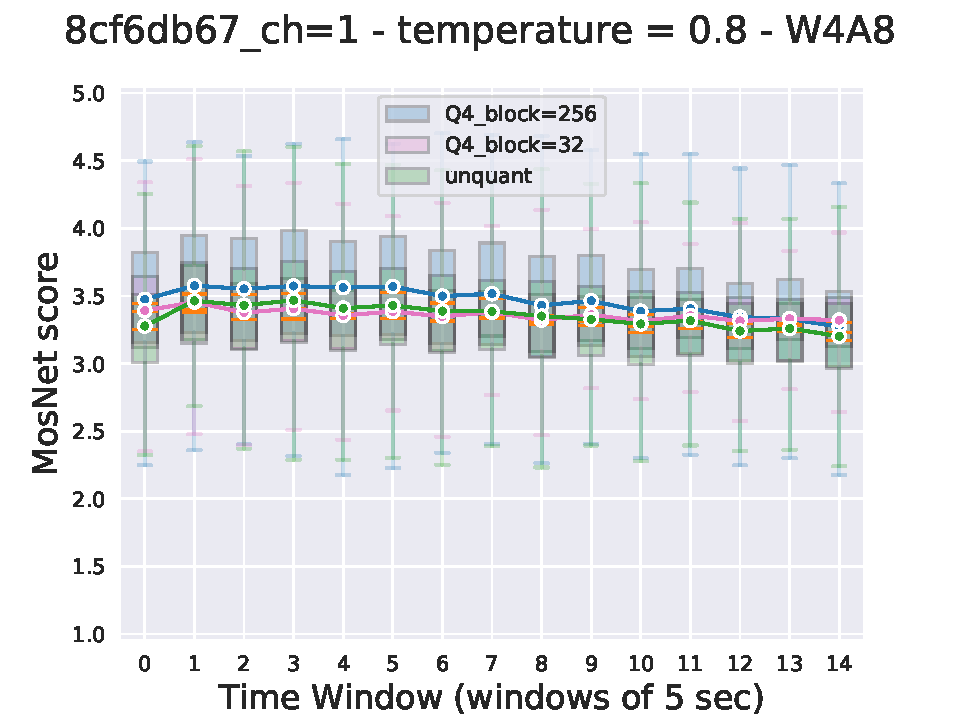
\includegraphics[height=0.275\linewidth, trim={0.6cm 0 1.7cm 0.9cm},clip]{figures/quantized_models_mosnet/codec_5bd939b7/mosnet_scores_8cf6db67_t=0.8_bits=4_5_ch=1.pdf}
\hfill
    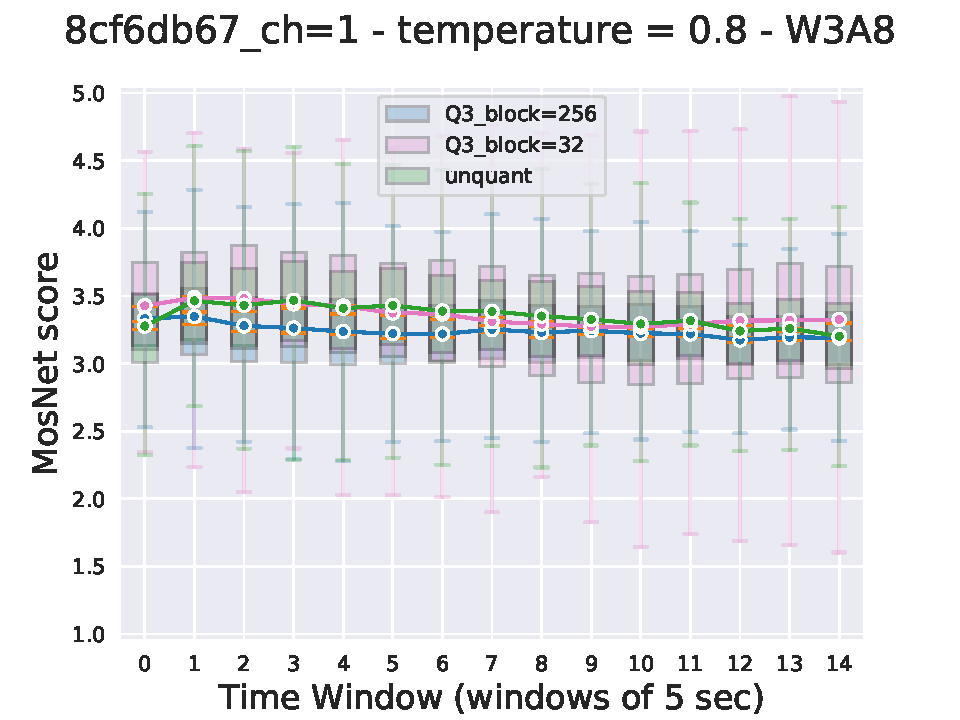
\includegraphics[height=0.275\linewidth, trim={1.8cm 0 1.7cm 0.9cm},clip]{figures/quantized_models_mosnet/codec_5bd939b7/mosnet_scores_8cf6db67_t=0.8_bits=3_5_ch=1.pdf}
\hfill
    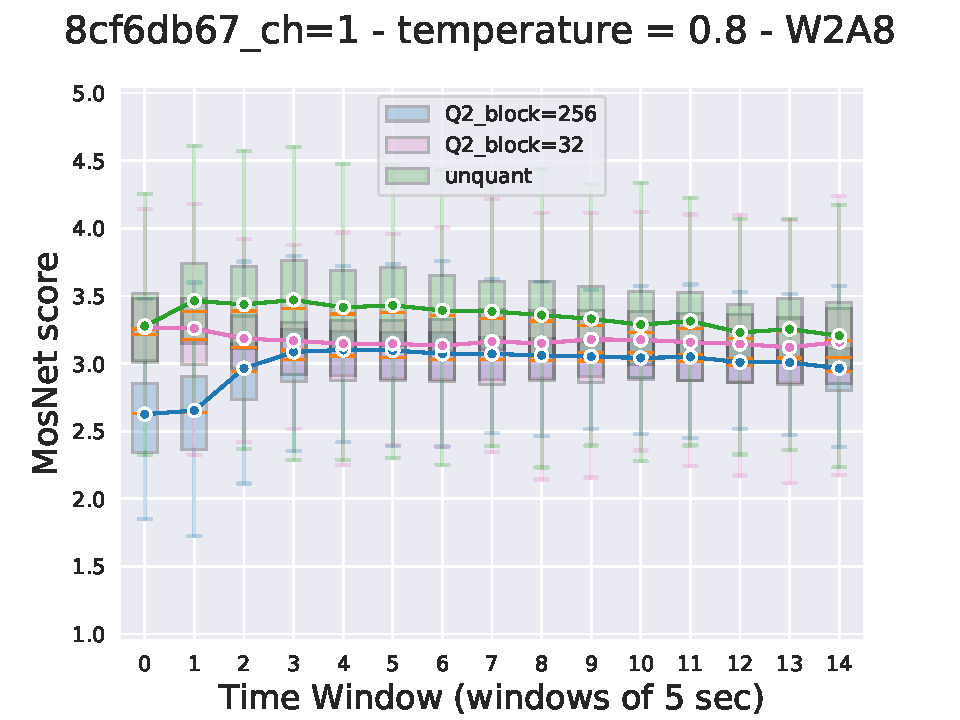
\includegraphics[height=0.275\linewidth, trim={1.8cm 0 1.7cm 0.9cm},clip]{figures/quantized_models_mosnet/codec_5bd939b7/mosnet_scores_8cf6db67_t=0.8_bits=2_5_ch=1.pdf}

\caption{\label{fig:quantmosnet}\textbf{Acoustic impact of model compression on \ours}. MOSNet evaluation of samples  generated by models compressed for different bitwidths. We evaluate the MOSNet scores across non overlapping windows of 5s, and report the distribution of these scores over 500 samples for each model.
}
\end{figure}




\begin{figure}[t]
~\bigskip \bigskip 

\centering
\begin{minipage}[t]{0.47\textwidth}
\scriptsize
   
    \centering
    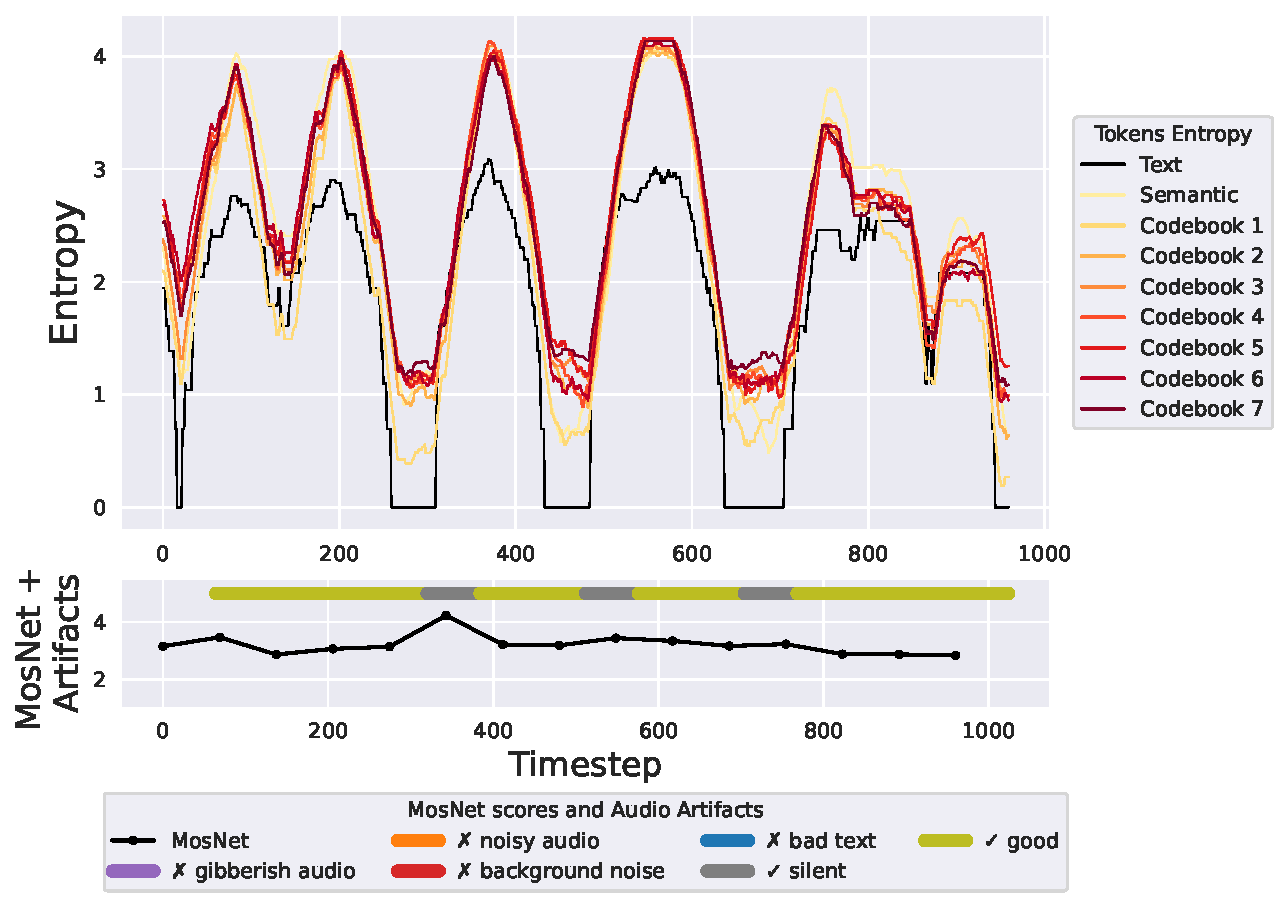
\includegraphics[width=\linewidth]{figures/quantized_models_mosnet/quant_artifacts_examples/good_sample_2.pdf}
    
    \textbf{(a)} Entropy spectrum of a well-behaved sample (no noticeable degradation). Short silences occur naturally in Moshi's output due to the model's multi-stream abilities (reflecting the other speaker's turn)

\end{minipage}
~~
\begin{minipage}[t]{0.47\textwidth}
\scriptsize
    \centering
    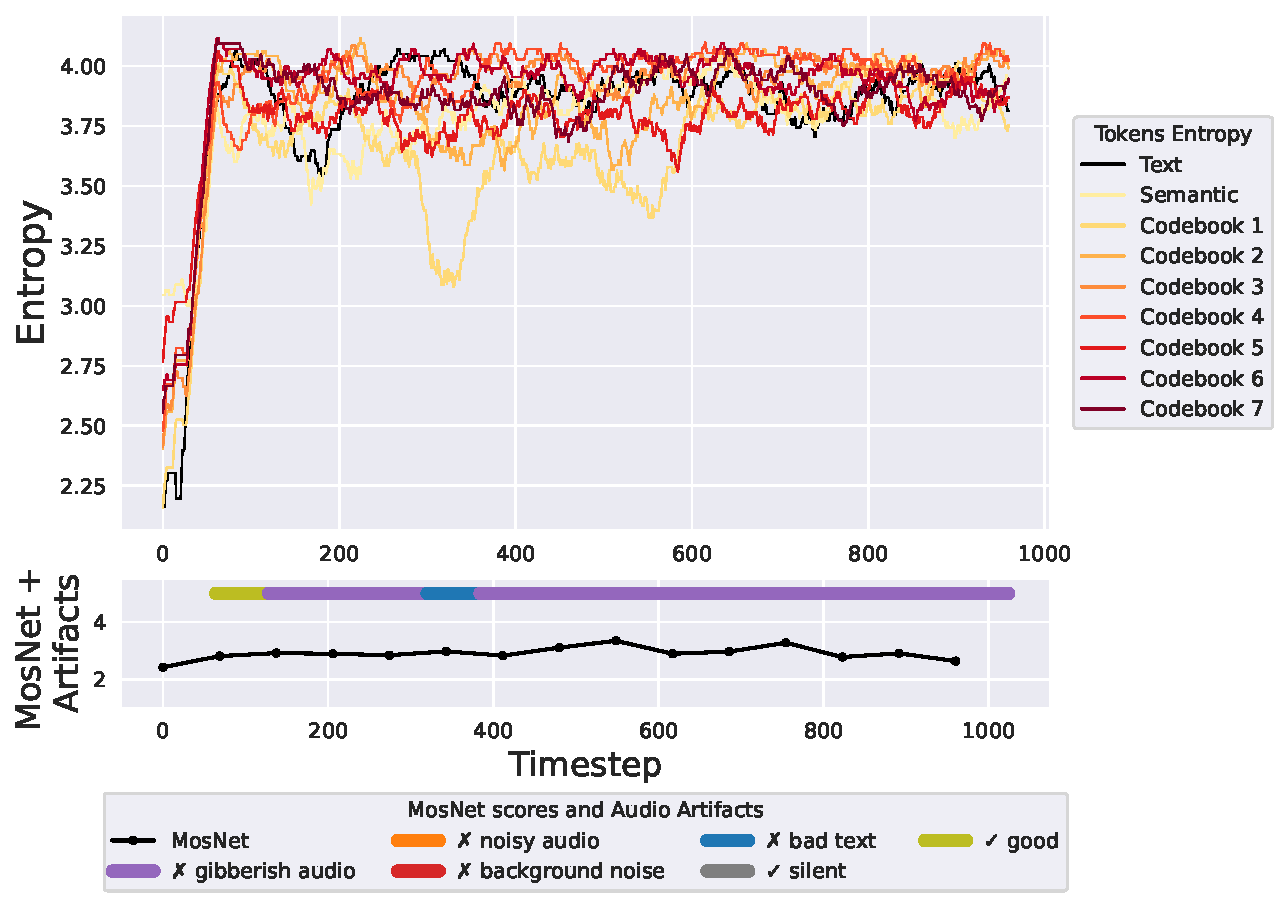
\includegraphics[width=\linewidth]{figures/quantized_models_mosnet/quant_artifacts_examples/W2_gibberish.pdf}
    \textbf{(b)} Significant degradations occur at low bitwidth (W2A8). These are not always well reflected by the MOSNet scores' magnitude, but  the entropy of the text token is visibly higher.
\end{minipage}
\caption{\label{fig:artifactsexample}\textbf{Audio artifacts caused by model compression}. Example of typical entropy spectrums capturing specific audio artifacts caused by model quantization. For each timestep, we compute the entropy over the past 128 tokens, independently for the text and audio codebooks tokens. Then, we measure the presence or absence of the different artifacts over non-overlapping windows of 64 tokens, as described in \hyperref[app:artifactsmetric]{Appendix \ref{app:artifactsmetric}}.}
\end{figure}

Following this insight, we measure the presence or absence of different audio artifacts on the same generated audio samples as the ones used in the previous MOSNet analysis. We report the results in \hyperref[tab:artifactssummary]{Table \ref{tab:artifactssummary}}, as well as a more detailed per timestep analysis in \hyperref[fig:artifacts]{Figure \ref{fig:artifacts}} of \hyperref[app:artifactsmetric]{Appendix \ref{app:artifactsmetric}}.
At a bitwidth of 4, we again observe little audio degradation.  
Decreasing to 3-bit format, audio degradations are more apparent and tend to become more frequent along the generation timestep, although the finer granularity quantization format is generally more robust to these artifacts. 
Nevertheless, both quantization formats display significantly degraded audio quality when weights are aggressively quantized to 2 bits, which we also observe qualitatively.

\begin{table}[t]
    \caption{\textbf{Distribution of audio artifacts caused by model compression}. Percentage of audio artifacts measured in the entropy spectrum of text and speech generated tokens, as described in \hyperref[app:artifactsmetric]{Appendix \ref{app:artifactsmetric}}. These results averaged across 500 samples generated by different versions of the same quantized Moshi, and across 16 timesteps of 64 tokens. Values of 0 \% are omitted in the table for better readability.}
    \label{tab:artifactssummary}
    \footnotesize
    \centering
    \begin{tabular}{lccccc}
        \toprule
        Model / Artifacts & Gibberish  & Noisy  & Background & Repetitive & No artifacts \\
         & audio & audio & noise &  text & \\
         \midrule
         unquant & & \ 4.1 & \ 0.1  &  \ 0.1 & 95.8 \\
         \midrule
         W4A8, block=32 & & \ 3.8  & \ 0.1  & \ 0.4 & 95.7 \\
         W4A8, block=256 & \ 0.1 & \ 3.7 &  & \ 2.2 & 94.0 \\
         \midrule
         W3A8, block=32 & \ 0.5 & \ 4.7 & \ 5.9 & \ 8.1 & 80.7 \\
         W3A8, block=256 & \ 0.2 & 12.2 & \ 3.1  & 21.9 & 62.7 \\
         \midrule
         W2A8, block=32 & 12.7 & 40.9 & \ 0.5 &  \ 0.4 & 45.4 \\
         W2A8, block=256 & 83.1 & & &  11.0 &  \ 5.9 \\
        \bottomrule
    \end{tabular}
\end{table}

\looseness=-1
\paragraph{Discussion.} The linguistic abilities of Moshi are more sensitive to quantizing the model weights and activations than its output audio quality.
More specifically, the audio quality remains close to that of the floating point baseline down to 4 bits precision, even when quantizing the full model, including the Depth Transformer. 
In contrast, the MMLU performance suffers significant drops when quantizing the model weights below 6 bits using post-training only quantization.
Following recent quantization techniques~\citep{quipsharp}, we may expect improved performance at lower bitwidth by using quantized aware finetuning  instead of PTQ. However, as Moshi's training pipeline from \hyperref[sec:maindatasets]{Section \ref{sec:maindatasets}} involves multiple stage and training datasets, this would require a more thorough investigation into designing quantized training phases and calibration datasets, to preserve all of \ours{}'s abilities lost after quantization.


